%preamble
\documentclass[letterpaper]{article}
\synctex=1

\usepackage{listings}
\lstset{
%language=Assembler
% breaklines=true
%frame=single,
%xleftmargin=-1pt
}
\usepackage{geometry}
\usepackage{array}
\usepackage{lipsum}

\usepackage{graphicx}
\usepackage{float}
\graphicspath{ {images/} }

\usepackage{float}

\usepackage[hidelinks]{hyperref}

% \usepackage[section]{placeins}
%
% \newenvironment{changemargin}[2]{%
% \begin{list}{}{%
% \setlength{\topsep}{0pt}%
% \setlength{\leftmargin}{#1}%
% \setlength{\rightmargin}{#2}%
% \setlength{\listparindent}{\parindent}%
% \setlength{\itemindent}{\parindent}%
% \setlength{\parsep}{\parskip}%
% }%
% \item[]}{\end{list}}

% \usepackage{tabu}
%actual document
\begin{document}

  %titlepage
  \begin{titlepage}
    \begin{center}

      \LARGE
      ECE 212 Lab - Introduction to Microprocessors

      Department of Electrical and Computer Engineering

      University of Alberta

      \vspace{2cm}

      Lab 3: Introduction to Subroutines

      \vspace{5cm}
      \Large

      \begin{tabular}{ | m{5cm} | m{5cm} | }
        \hline
        Student Name & Student \\
        \hline
        Arun Woosaree & XXXXXXX \\
        \hline
        Navras Kamal & 1505463 \\
        \hline
      \end{tabular}


      % \begin{tabu} to 0.8\textwidth{  | X[c] | X[c] | }
      %   \hline
      %   Student Name & Student \\
      %   \hline
      %   Arun Woosaree & xxxxxxx \\
      %   \hline
      %   Navras Kamal & 1505463 \\
      %   \hline
      % \end{tabu}


    \end{center}
\end{titlepage}

%table of tableofcontents

\tableofcontents

% \vfill
\newpage

\section{Introduction}
This lab deals with stack operation (push and pop), segmenting a long program/function into several smaller and simpler subroutines/sub-functions. … ….


  \subsection{Part A}
  In part A, ......
  \subsection{Part B}
  For part B, ......
  \subsection{Part C}
  \textbf{FILLINTHEINTRO}

  The purpose of this lab is to learn and test with the Assembly language in a hands on environment
  in order to solidify the concepts learned in class and to improve our skill in the language.  In
  addition, we will be learning how to handle the Netburner ColdFire boards directly, manipulating
  the contents of their memory and data structures.  Finally, we are going to learn how to work inside
  the Eclipse IDE environment and how to properly use the powerful tools that come alongside it.



  The code will be developed for the Netburner ColdFire Platform, which has some parameters that should
  be kept in mind throughout testing.  There are multiple Data and Address registers, and the memory
  is indexed by hexadecimal codes.  The data and the stored locations can each be modified directly, values
  can be compared and the code can branch into different sections depending on the values of the CCR
  (Condition Code Register) bits,
  which store information about the outcome from the last comparison or valid operation, such as if a
  value is negative or zero.  These will be used to execute code conditionally.

  The lab will be split into two sections, each with a different goal but with similar implementations.
  For one part we will be taking in an ASCII value and if the character it represents is a character
  included in the symbols for hexadecimal numbers then that hexadecimal value is output, otherwise
  it returns an error.  For the second part an ASCII value is taken in, and if the character it represents
  is a letter in the English language (A-Z) then the ASCII code for the character in the opposite case
  is output.  Thus, valid uppercase English letters are converted to their lowercase equivalents in ASCII
  and vice versa.


  These experiments will introduce implementing high level programming practices of loops, if - then - else statements,
  using the Assembly language. More specifically, this will introduce the movement of
  memory and data to and from different parts of the Netburner chip, using techniques such as referencing
  memory addresses and copying data to local data registers.  The debugger tools of the IDE will be used
  to closely examine this movement and to analyze all changes to the data in order to solve issues in
  development as well as to test the code.  This is all building off the concepts explored in Lab 0.

  The computing science practice of Pair Programming was also introduced, where two people
  develop and test code in tandem.  The partners are divided into the Driver and the Navigator.
  In this structure the Driver is the one responsible for the physical typing of the code into the computer,
  and the Navigator reviews this code and clarifies the meaning of each passage in order to find bugs faster
  and to improve efficiency in testing.  The two partners should communicate constantly and switch in order
  to maximize the efficiency of this working model.  This will not only decrease time needed for development
  but it will also improve the quality of code from each partner.


\section{Design}
  \subsection{Part A}
    For the first part of the lab, we begin by writing our own subroutine.
    Some code was already supplied such that:
    \begin{itemize}
      \item Stack Entry Condition =
        \begin{enumerate}
          \item Space allocated for the number of entries on stack (long word)
          \item Space allocated for the divisor number on stack (long word)
        \end{enumerate}
      \item Stack Exit Condtion =
        \begin{enumerate}
          \item Number of entries on stack (long word)
          \item Divisor number on stack (long word)
        \end{enumerate}
    \end{itemize}

    \begin{figure}[h!]
      \centering
      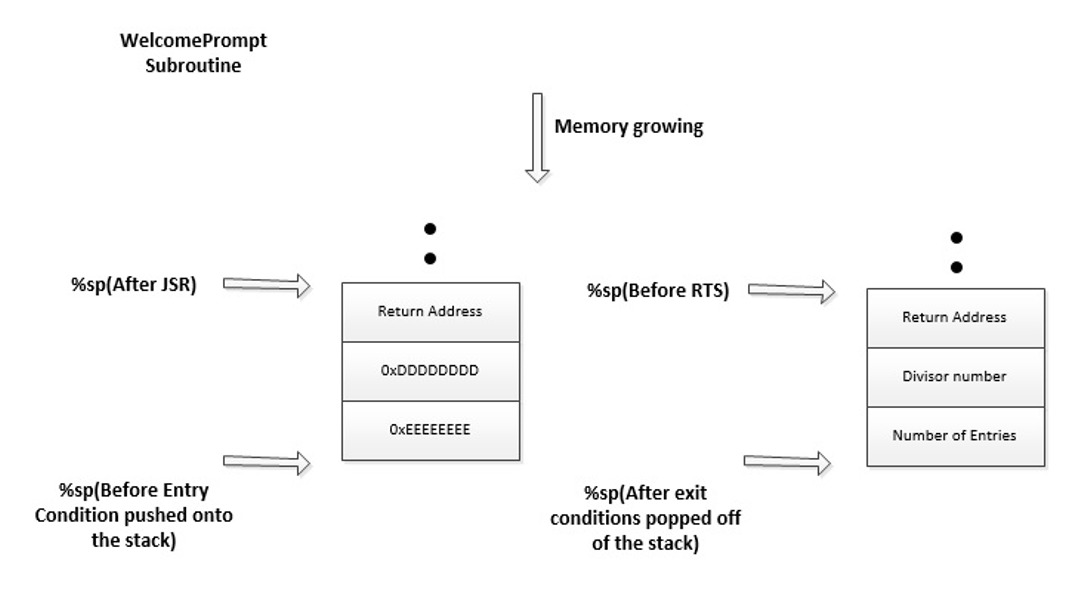
\includegraphics[width=.8\textwidth]{designa.jpg}
      \caption{Visualization of the stack for Part A}
    \end{figure}

    We started by editing \textit{Lab3a.s}, and chose to back up
    address registers \textit{a2-a6} and the data registers d2-d7. Since the stack pointer
    was \textit{a7}, this was accomplished by subtracting 44 from the stack pointer,
    then using a MOVEM.L command to push the values onto the stack. Then at the end, just before
    the RTS command in the subroutine, we move the values we backed up to the registers
    as they were before running the subroutine. Address register \textit{a2} was chosen to
    hold the memory location of where the valid numbers which were entered would go, which
    was 0x2300000.
    Next, at the very end of the file, we
    defined several messages as strings that would be used as prompts. Labels are used to reference
    these strings, which are used for prompting the user in the MTTTY serial monitor to enter relevant data for each part.

    With the initial setup for this subroutine completed, we moved on to
    actually coding the prompt messages for the program. We begin by
    pushing the Welcome Prompt onto the stack, and using the provided \textit{iprintf}
    and \textit{cr} subroutines to print the Welcome Message and a carriage return for the
    user. Once the message was displayed, we immediately clean up the stack by adding 4
    to the stack pointer, since the address of the message was pushed onto the stack,
    and addresses take up 4 bytes of memory. For every message printed onwards,
    we immediately clean up the stack after the message is printed. We then branch to a label where the user
    is prompted to enter the number of entries. The subroutine getstr, which was provided captures input from the serial monitor,
    and puts it into data register \textit{d0}. For this part, the only
    valid entries are the numbers 3-15, with anything else entered being rejected.
    This was accomplished by comparing the input to the number 15. If the number was
    greater than 15. we branch to a label to warn the user that an invalid entry was entered,
    and then the program returns to the label which prompts the user to enter
    the number of entries. Similarly, if the value entered was less than 3, the same thing would occur.
    If the entry was valid, we put the numentries value that the user entered in the spot reserved on the
    stack for us. This value was also copied to \textit{d7}, which is later used as a counter
    for when the user enters the numbers. As a feature for the user, if the input was
    accepted, the value is printed to the serial monitor for the user to see. This is done
    in a similar method to how the messages are printed onto the stack.

    In a very similar fashion, the user is then prompted to enter the divisor number.
    Here, the accepted values were from 2-5, with the data validation checks happening in
    almost exactly the same was as outlined above for entering the number of entries.
    The divisor also went into a spot on the stack, which was reserved for us.

    Next, we enter a loop, where the user is prompted to enter numbers, until
    the user enters as many numbers as the user declared when prompted to enter the number of entries.
    The loop itself loops numentries-1 times, since there's a different prompt message for the
    last number. As mentioned earlier, we use \textit{d7} as our counter, since numentries was
    copied to this data register. The user then goes through the same process of
    entering numbers, and is prompted to re-enter the number if it is not positive.
    This is done similarly to above, in that the number entered is compared to the
    number 1, and if the number entered is less than 1, we branch to a label where
    the user is warned about the mistake, and then branches back to continue the loop.
    If the number is accepted, then it is printed to the serial monitor, and then the
    number entered is moved to the address location pointed to by \textit{a2}, and \textit{a2} is post
    incremented. On each successful loop iteration, the number 1 is subtracted from
    the counter \textit{d7}, until the counter is 1.

    At this point, the user needs to enter one last number, for which there is
    an appropriate prompt, and the data validation is the exact same as above,
    with only positive values being accepted. If the number is valid, then it is
    printed to the serial monitor, and moved to the memory location where \textit{a2} points.

    Finally, we reach the part where the backed up registers on the stack are restored,
    and the subroutine hits the RTS command.

    % \subsubsection{Part A Sample Calculations of Conversion}
    %
    %     input = `9' = 0x39\\
    %     0x39 - 0x30 = 0x9\\
    %     \\
    %     input = `E' = 0x45\\
    %     0x45 - 0x41 = 0x4\\
    %     0x4 + 0xA = 0xE\\
    %     \\
    %     input = `d' = 0x64\\
    %     0x64 - 0x61 = 0x3\\
    %     0x3 + 0xA = 0xD

  \subsection{Part B}
    In Part B, another subroutine is written, which computes some stats
    on the numbers entered. Similar to Part A, some code was provided
    such that the stack entry and exit conditions are as follows:

    \begin{itemize}
      \item Stack Entry Condition =
        \begin{enumerate}
          \item Space allocated for how many numbers are divisible by the divisor (long word)
          \item Number of entries (long word) on stack
          \item Divisor number (long word) on stack
        \end{enumerate}
      \item Stack Exit Condtion =
        \begin{enumerate}
          \item How many numbers are divisible by the divisor (long word) on stack
          \item Number of entries on stack (long word)
          \item Divisor number on stack (long word)
        \end{enumerate}
    \end{itemize}

    \begin{figure}[h!]
      \centering
      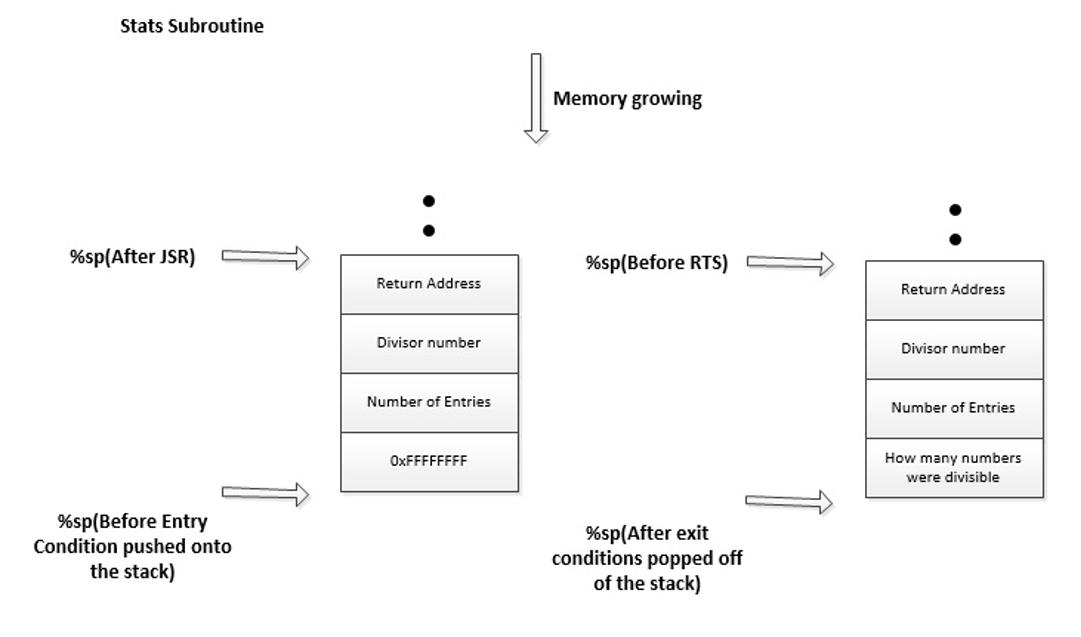
\includegraphics[width=.8\textwidth]{designb.jpg}
      \caption{Visualization of the stack for Part B}
    \end{figure}

    We begin by backing up the registers $a0-a6$ and $d0-d7$ by
    subtracting 60 from the stack pointer, and then using the \textit{movem}
    command to push those values onto the stack. Similarly, at the end of the
    subroutine just before rts, we restore the values by using \textit{movem} to restore the values,
    then add 60 to the stack pointer before returning to the previous subroutine.

    We begin by reading the numentries and divisor off of the stack, which
    were put there by the subroutine in Part A. The addresses 0x2300000
    and 0x2310000 were loaded into address registers \textit{a2} and \textit{a3} respectively.
    \textit{a2} kept track of the location were the numbers were entered, and \textit{a3}
    kept track of where the min, mean, max, and divisible numbers would be output.

    To begin calculating the minimum number, we copy the numentries to another
    data register to use as a counter. The first number is read by indirectly addressing
    \textit{a2} with a post increment, and moved to a data register which will hold the
    final minimum value. Inside a loop, which loops numentries-1
    times, (since the first number was already read), the next number is read by indirectly
    addressing \textit{a2} with a post increment, and
    moved into a temporary data register, where it is then compared to the data register
    which is supposed to hold the minimum value. If the temporary value is less than the
    minimum value, we move the temporary value to the data register which holds the minumum value.
    If the temporary value is greater than the current minimum, then the loop continues.
    At the end of every loop iteration, the loop counter is decremented by 1, and compared
    to the number 1, since it loops numentries-1 times. Once this loop is complete,
    the minumum value is stored in data register \textit{d5}, so we move it to
    the memory location pointed at by \textit{a3} and post increment it.

    The maximum number is calculated in a very similar manner compared to how
    the min was calculated. First, \textit{a2} is reset to 0x2300000, and the loop counter
    is reset to numentries, since we post
    incremented \textit{a2} when finding the min, and we decremented the counter
    when going through the numbers again to find the min.
    Then, we go through a loop that is almost the same as for calculating the minumum number.
    except that the current maximum number is held in one data register,
    and a temporary value is read and compared to the maximum number. If the temporary
    number is greater than the current maximum, then the temporary number becomes the
    maximum, and by the end of the loop, the maximum value is stored in data register \textit{d6},
    so we move it to
    the memory location pointed at by \textit{a3} and post increment it.

    To find the mean, address register \textit{a2} was reset to 0x2300000,
    and the loop counter was reset to numentries again. A data register was used
    to store the cumulative sum of the numbers, which was accomplished by
    first clearing the data register, then looping over the list of
    numbers entered (pointed at by \textit{a2}), and adding each number
    to the sum. This was done by indirectly addressing \textit{a2} with
    a post increment to copy the value to a data register, then adding
    that value to our cumulative sum. At the end of the loop, we have the
    cumulative sum, so to
    find the mean, we simply divide the cumulative sum by the numentries
    by using \textit{divs.l}. When the division was complete, the
    mean was stored in data register \textit{d4}, so so we move it to
    the memory location pointed at by \textit{a3} and post increment it.

    Finally, to find the divisible numbers, we once more reset \textit{a2}
    to 0x2300000, and the loop counter to numentries. We go through one last loop,
    where a number is read by indirectly addressing \textit{a2}, moving it to
    a data register, and then using \textit{divs.w} to divide the number by the
    divisor, since \textit{divs.w} provides the remainder stored in the
    16 most significant bits. If the number is divisible, it
    should not have a remainder, so we check the remainder by
    bit shifting the division result 16 bits to the right, and check if
    the remainder is 0. If so, a counter which holds the number of
    divisible numbers is incremented by 1, and the divisible number
    is moved to the location pointed at by \textit{a3} and post incremented.
    The loop then continues until all the numbers have been processed. At the
    end of the loop, the number of divisible entries is stored in data register \textit{d7},
    so we move it to the spot reserved on the stack for us.

    We then reach the end of the subroutine, where we restore the backed up register values
    on the stack, add 60 to the stack pointer, and return to the previous subroutine.


    \subsubsection{Sample Calculations}
    Numbers entered: 1,2,3,4,5\\
    Numentries: 5\\
    Divisor: 2\\ \\
    Min: 1\\
    Max: 5\\
    Mean: $\frac{1+2+3+4+5}{5}=3$\\
    Numdivisible: 2\\
    Divisible numbers: 2,4


    \subsection{Part C}

    In Part C, the last subroutine is written, which prints the stats
    on the numbers entered. Similar to the previous parts, some code was provided
    such that the stack entry and exit conditions are as follows:

    \begin{itemize}
      \item Stack Entry Condition =
        \begin{enumerate}
          \item How many numbers were divisible by the divisor
          \item Number of entries (long word)
          \item Divisor number (long word)
        \end{enumerate}
      \item Stack Exit Condtion =
        \begin{enumerate}
          \item How many numbers are divisible by the divisor
          \item Number of entries (long word)
          \item Divisor number (long word)
        \end{enumerate}
    \end{itemize}

    \begin{figure}[h!]
      \centering
      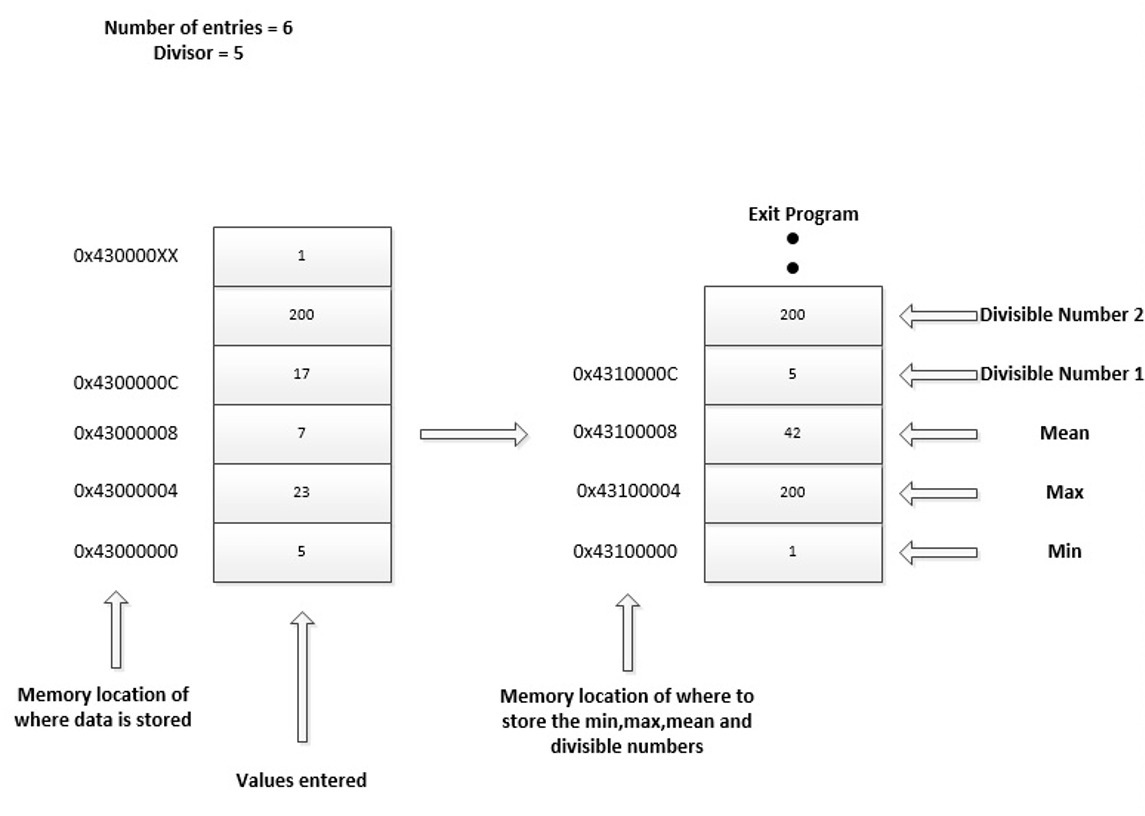
\includegraphics[width=.8\textwidth]{designc.jpg}
      \caption{Visualization of the stack for Part A}
    \end{figure}

    Just like in part B, we begin by backing up the registers $a0-a6$ and $d0-d7$ by
    subtracting 60 from the stack pointer, and then using the \textit{movem}
    command to push those values onto the stack. Similarly, at the end of the
    subroutine just before rts, we restore the values by using \textit{movem} to restore the values,
    then add 60 to the stack pointer before returning to the previous subroutine.
    We begin by loading 0x2300000 into \textit{a2}, 0x2310000 into \textit{a3},
    and the divisor, numentries, and numdivisible are read from the stack and
    moved into data registers.

    At the very end of the program, we define strings just like
    in Part A, which are printed for the user to read.
    We begin by first printing the number of entries.
    A message is printed by pushing the address of a string defined earlier
    onto the stack, and using \textit{iprintf}. Next, the actual
    number of entries is pushed onto the stack and printed to the
    serial monitor using the subroutine \textit{value}. The stack is also cleaned up by
    adding to the stack pointer. The user is then prompted that the numbers will
    be printed, which is done in a very similar manner, using \textit{iprintf}. Then,
    a loop iterates over the numbers, which are indirectly addressed with \textit{a2} with post increment,
    and printed with the subroutine \textit{value}. The data register holding the numentries
    is decremented at the end of each iteration of the loop, until it reaches 0, which is
    when all the numbers have been printed. The min, max, mean, and number of divisible numbers are all printed
    in a similar manner to how the numentries was printed, with a message
    printed first using \textit{iprintf}, and then the value being printed
    with the subroutine \textit{value}. Whenever something is printed, the stack is
    immediately cleaned up afterwards by adding 4 to the stack pointer whenever a value is printed.

    Finally, in a manner similar to how the numbers were printed, the
    divisible numbers are printed by indirectly addressing \textit{a3} with post
    increment, putting the number on the stack, and jumping to the subroutine
    \textit{value} to print the numbers. This happens in a loop, with numdivisible
    being decremented at the end of each loop iteration, until all the
    divisible numbers are printed out.

    At the end of the subroutine, the string ``End of program'' is printed
    to let the user know that the program has ended.  

\section{Testing}
  \subsection{Part A}
    Initially, we visually tested our code by using the debugger in Eclipse IDE.
    While stepping through the code, we would check the values at relevant memory
    locations, and the data and address registers. When the bugs were ironed out,
    we went on to the next phase of testing.
    Our code was tested using the provided \textit{Lab1Test.s} file. More specifically,
    this program was moved into the project folder, downloaded to the ColdFire microcontroller,
    and the MTTTY serial monitor was loaded to monitor the expected output. Our code was
    further tested by replacing the `DataStorage.s' file with the other variants provided
    named: \textit{DataStorage1.s}, \textit{DataStorage2.s}, and \textit{DataStorage3.s}.
    Finally, our program, which produced the correct output, was verified by a lab TA.

    \begin{figure}[H]
      \centering
      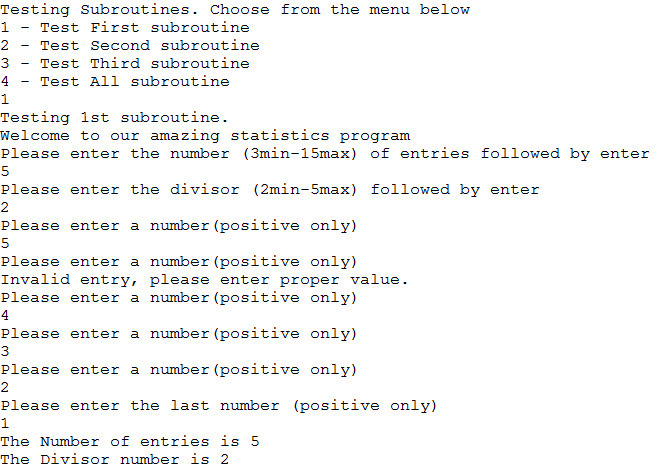
\includegraphics[width=0.4\textwidth]{parta.jpg}
      \caption{MTTTY output when testing our Part A solution}
    \end{figure}

  \subsection{Part B}
    The procedure for testing our code for part B was very similar to the process
    described above in Part A. We visually inspected our code in the Eclipse IDE,
    used the Eclipse debugger to step through our code, and monitor relevant
    memory addresses and registers. When we were confident that we had a working
    solution, we used the provided files \textit{Lab1Test.s}, and the \textit{DataStorage*.s}
    files to verify our solution by downloading the program to the ColdFire microcontroller,
    and monitoring the output in MTTTY. Finally, our solution was verified by a lab TA.

    \begin{figure}[H]
      \centering
      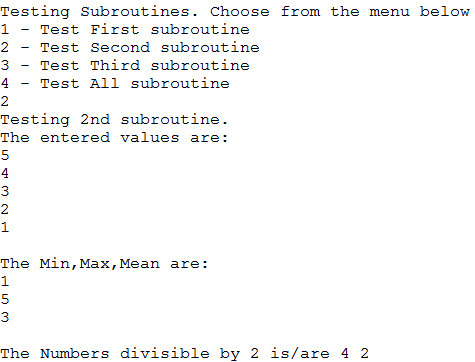
\includegraphics[width=0.4\textwidth]{partb.jpg}
      \caption{MTTTY output when testing our Part B solution}
    \end{figure}

    \subsection{Part C}
      The procedure for testing our code for part C was very similar to the process
      described above in Part A. We visually inspected our code in the Eclipse IDE,
      used the Eclipse debugger to step through our code, and monitor relevant
      memory addresses and registers. When we were confident that we had a working
      solution, we used the provided files \textit{Lab1Test.s}, and the \textit{DataStorage*.s}
      files to verify our solution by downloading the program to the ColdFire microcontroller,
      and monitoring the output in MTTTY. Finally, our solution was verified by a lab TA.

      \begin{figure}[H]
        \centering
        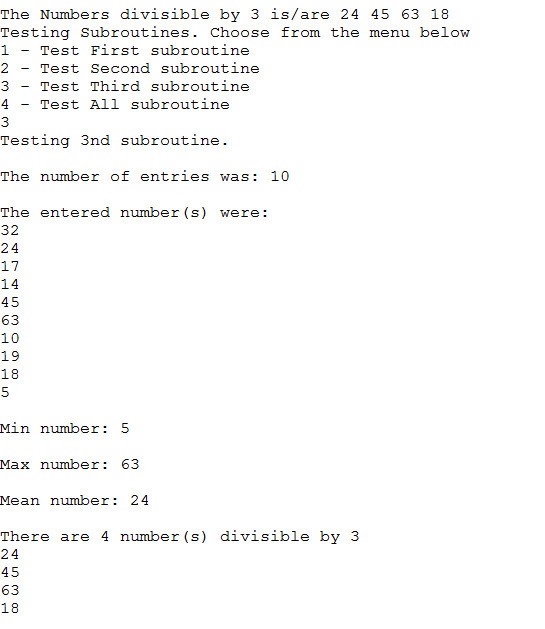
\includegraphics[width=0.4\textwidth]{partc.jpg}
        \caption{MTTTY output when testing our Part B solution}
      \end{figure}

      \begin{figure}[H]
        \centering
        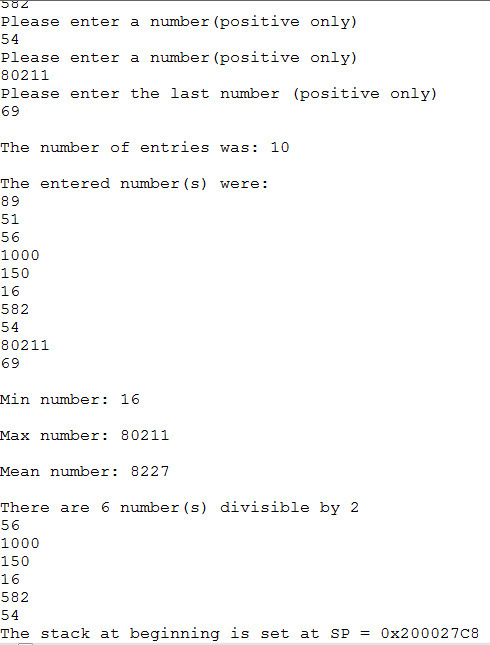
\includegraphics[width=0.4\textwidth]{allparts.jpg}
        \caption{MTTTY output when testing our Part B solution}
      \end{figure}

\section{Questions}

    \subsection{Question 1}
      \textit{Is it always necessary to implement either callee or caller preservation of registers when calling a subroutine. Why?}
      \\ \\
      \noindent\textbf{A:}
      % \lipsum[7]
      Yes. This would cause a problem, because there would be no way to exit the program,
      so the program would keep reading data and moving the converted values to
      memory locations, until the program attempts to read or write to a memory
      location that is restricted or non-existant. This would then cause the
      program to crash.

    \subsection{Question 2}
      \textit{Is it always necessary to clean up the stack. Why?}
      \\ \\
      \noindent\textbf{A:}
      % \lipsum[8]
      Assuming the data range would be fixed and hardcoded into the Assembly code it would be possible to
      write the max range (ie. 10) into an unused data register such as \%d3.  Then, instead of checking
      for the enter code on each iteration where there is an invalid value, we could check the value stored in
      \%d3 before checking the validity of the value stored in the current memory address.  If \%d3 is
      zero then jump to the \textbf{end} label, breaking the loop.  Another way to do it would be again
      to assume that the number of iterations is fixed and the size of data being checked is fixed as being
      long-words would be to check the value of the memory address stored in (\%a1) after each iteration
      before returning to the beginning of the loop and after the memory addresses have been incremented.
      If at that point the memory address is [(initial memory address 0x2300000) + (0x4 * N)], where N is
      the number of desired iterations (this value would be hardcoded, this is just a general case), then
      jump to the \textbf{end} label, breaking the loop.  This way would be more memory efficient as it
      does not require an additonal data register and the modification of a counter value.  Thus it isn't always necessary, though it is usually good practice regardless

      \subsection{Question 3} \textit{If a proper check for the getstring
      function was not provided and you have access to the buffer, how would you
      check to see if a valid \# was entered? A detailed description is
      sufficient. You do not need to implement this in your code.
      \\ \\
      ``Hello Students,
		In question no. 3, you are asked to answer the following:
		You have to describe how you are going to check that the entered number is valid or not.
		For example, one entry is say 409 and another is 4h9. Here, 4h9 is a wrong number. Now please explain how are you going to check that?
		Thanks.''}

      \noindent\textbf{A:}
        % \lipsum[8]
        Assuming the data range would be fixed and hardcoded into the Assembly code it would be possible to
        write the max range (ie. 10) into an unused data register such as \%d3.  Then, instead of checking
        for the enter code on each iteration where there is an invalid value, we could check the value stored in
        \%d3 before checking the validity of the value stored in the current memory address.  If \%d3 is
        zero then jump to the \textbf{end} label, breaking the loop.  Another way to do it would be again
        to assume that the number of iterations is fixed and the size of data being checked is fixed as being
        long-words would be to check the value of the memory address stored in (\%a1) after each iteration
        before returning to the beginning of the loop and after the memory addresses have been incremented.
        If at that point the memory address is [(initial memory address 0x2300000) + (0x4 * N)], where N is
        the number of desired iterations (this value would be hardcoded, this is just a general case), then
        jump to the \textbf{end} label, breaking the loop.  This way would be more memory efficient as it
        does not require an additonal data register and the modification of a counter value.

\section{Conclusion}
  This lab demonstrated how to perform operations
  and modify data while moving it around using the Assembly language for the ColdFire architechture.
  In addition, the lab improved our understanding of the debugger software, a very powerful
  tool in the development of this kind of code.  The main issue we found was related
  to the hardware itself, as there was some instances where the code did not execute
  properly and the board itself needed to be reset.  The other issue we faced was mostly
  around getting used to the software and the workflow in the Eclipse IDE and
  the debugger.  Once we understood the ways to use the tools we found our workflow sped up
  considerably, as we were able to check step by step and find bugs at the source.  The last
  issue we had was with the syntax of the code, but that was solved quickly by reading over
  documentation and with the help of the TAs.  Overall the lab went smoothly and has indeed
  succeeded at the goals of improving our familiarity and skill with the Netburner ColdFire system,
  Assembly code and Pair Programming practices.

\newpage
\section{Appendix}
  %\textwidth=600pt
  \subsection{Part A Assembler Code}
    % \begin{changemargin}{-2cm}{-2cm}
    \lstinputlisting{code/Lab3a.s}
  % \end{changemargin}
\newpage
  \subsection{Part A Flowchart Diagram}
    \vspace{2cm}
    \noindent\makebox[\textwidth]{
\includegraphics[width=\paperwidth,height=.6\paperheight,keepaspectratio]{partaflowchart.jpg}}
\newpage
  \subsection{Part B Assembler Code}
    \lstinputlisting{code/Lab3b.s}
\newpage
  \subsection{Part B Flowchart Diagram}
  \vspace{2cm}
    \noindent\makebox[\textwidth]{
\includegraphics[width=\paperwidth,height=\paperheight,keepaspectratio]{partbflowchart.jpg}}
\newpage
\subsection{Part C Assembler Code}
  % \begin{changemargin}{-2cm}{-2cm}
  \lstinputlisting{code/Lab3c.s}
% \end{changemargin}
\newpage
\subsection{Part C Flowchart Diagram}
  \vspace{2cm}
  \noindent\makebox[\textwidth]{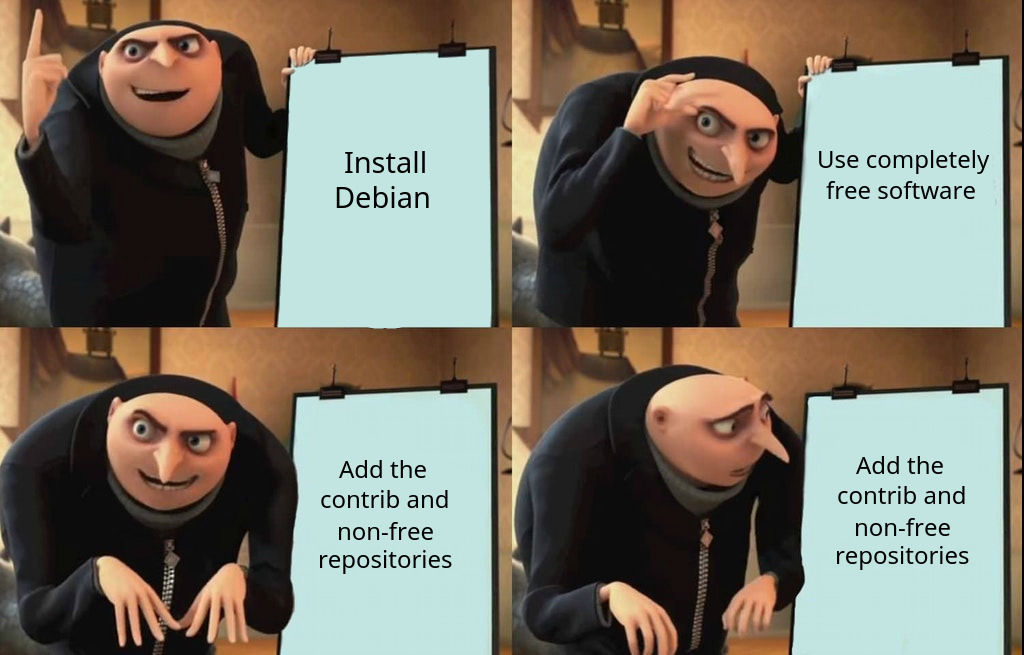
\includegraphics[width=\paperwidth,height=\paperheight,keepaspectratio]{partcflowchart.jpg}}
\newpage
% \pagenumbering{gobble}
% \addcontentsline{toc}{section}{Marking Sheet}
% \section{Marking Sheet}
% \clearpage
\addtocounter{section}{1}
% \addcontentsline{toc}{section}{Marking Sheet}
\addcontentsline{toc}{section}{\protect\numberline{\thesection} Marking Sheet}

\section{Marking Sheet}
\end{document}
